
\section{Producto Cartesiano}

Un conjunto es solo eso, una colección de objetos, pero no tiene ninguna estructura interna, ni siquiera un orden.
Necesitamos definir objetos más elaborados.

\vspace{.2cm}

\begin{defn}
Dados dos objetos  $x$ y $y$, se define un \emph{par ordenado}, a través de la notación $(x,y)$.

En éste se distingue la \emph{primera componente}: $x$, y la \emph{segunda componente}: $y$.

Dos pares ordenados $(a,b)$ y $(x,y)$ se dicen iguales si y solo si $a=x$ y $b=y$.
\end{defn}

De la definición de par ordenado se deduce que el orden en que aparecen es importante, no es lo mismo $(1,2)$ que $(2,1)$; por la misma razón, un par ordenado admite repeticiones, por ejemplo $(1,1)$ es un par ordenado legítimo.

En la notación de par ordenado es fundamental el uso de paréntesis redondos``('' y ``)'', en lugar de llaves ``$\{$'' y ``$\}$'', este solo detalle los diferencia de un conjunto, indicando que en este caso se trata de un objeto donde el orden en que aparecen los elementos sí es relevante.

A partir de esta noción, definimos una nueva operación entre conjuntos: el producto cartesiano, que consiste en todos los pares ordenados posibles de formar de un conjunto a otro.

\vspace{.2cm}


\begin{defn}
Dados dos conjuntos $A$ y $B$, se define un conjunto, llamado \emph{producto cartesiano de $A$ con $B$: $A\times B$}, como sigue.
$$A\times B=\{(a,b)\ :\ a\in A\textrm{ y } b\in B\}$$
\end{defn}


\begin{ejemplo}
El plano cartesiano se puede ver como el producto cartesiano de $\R$ consigo mismo: $\R\times \R$, ya que sus elementos, los puntos, están dados por sus dos coordenadas $(x,y)$.
\end{ejemplo}

Probablemente la mejor manera de visualizar el producto cartesiano entre dos conjuntos es justamente colocando uno de los conjuntos de manera horizontal y el otro de manera vertical y trazar líneas verticales y horizontales partiendo de ellos. Los puntos de intersección de las rectas conforman el producto cartesianos de los dos conjuntos.

\vspace{.2cm}


\begin{ejemplo}
Considerando $A=\{\heartsuit,\diamondsuit,\spadesuit\}$, $B=\{\heartsuit,\clubsuit\}$, resulta:
$$A\times B=\{(\heartsuit,\heartsuit),(\heartsuit,\clubsuit),(\diamondsuit,\heartsuit),(\diamondsuit,\clubsuit),(\spadesuit,\heartsuit),(\spadesuit,\clubsuit)\}.$$
Podemos visualizarlo con la siguiente figura.
\vspace{.5cm}
\begin{center}
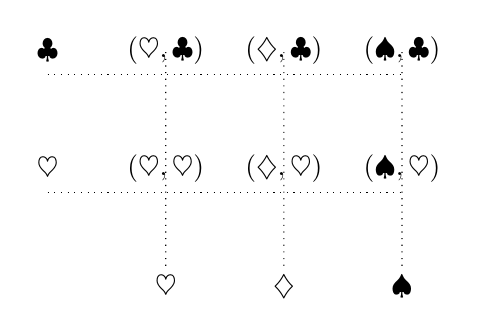
\begin{tikzpicture}[scale=1.5]
\node (A) at (1,0) {$\heartsuit$};
\node (B) at (2,0) {$\diamondsuit$};
\node (C) at (3,0) {$\spadesuit$};

\node at (1,1) {$(\heartsuit,\heartsuit)$};
\node at (2,1) {$(\diamondsuit,\heartsuit)$};
\node at (3,1) {$(\spadesuit,\heartsuit)$};

\node at (1,2) {$(\heartsuit,\clubsuit)$};
\node at (2,2) {$(\diamondsuit,\clubsuit)$};
\node at (3,2) {$(\spadesuit,\clubsuit)$};

\node (D) at (0,1) {$\heartsuit$};
\node (E) at (0,2) {$\clubsuit$};

\draw[dotted] (A) -- (1,2);
\draw[dotted] (B) -- (2,2);
\draw[dotted] (C) -- (3,2);
\draw[dotted] (0,0.8) -- (3,0.8);
\draw[dotted] (0,1.8) -- (3,1.8);
\end{tikzpicture}
\end{center}
\end{ejemplo}


\section{Funciones}

Las funciones son las ``máquinas'' más importantes de las que dispone la ingeniería para modelar y trabajar con el mundo. 
Las estudiaremos lentamente a través de todo el primer y segundo año de la carrera.

\vspace{.2cm}


\begin{defn}
Dados dos conjuntos $A$ y $B$, una función de $A$ en $B$ es un subconjunto $F\subseteq A\times B$ tal que para cada $x\in A$, existe un único $y$ en $B$ tal que $(x,y)\in F$; o simbólicamente:
$$\forall c\in A,\ \exists! y\in B,\ (x,y)\in F.$$
El elemento $y$ depende de $x$, y lo llamamos \emph{imagen de $x$}.
Dado que es único, decimos que la función $F$ \emph{asigna} a $x$ la imagen $y$, y escribimos 
$$F(x)=y,$$
donde normalmente daremos una fórmula de definición de $F$ que permitirá calcular $y$ a partir de $x$.
El conjunto $A$ se llama \emph{conjunto de partida} o \emph{dominio}, mientras que el conjunto $B$ se llama \emph{conjunto de llegada}.
Dada esta asimetría se prefiere denotar la función mediante la escritura siguiente:
$$ F:\ A\longrightarrow B.$$

Un subconjunto $F\subseteq A\times B$ cualquiera se llama \emph{relación}.
\end{defn}

\begin{ejemplo}\label{eje:C}
Consideremos $C:\R\rightarrow \R$ definida por $C(a)=a^4-2$.
Su gráfico será el siguiente.
\begin{center}
\begin{tikzpicture}[domain=-1.6:1.6]
\draw[arrows=->] (-4.2,0) -- (4.2,0) node[right] {$\R$};
\draw[arrows=->] (0,-4.2) -- (0,4.2) node[above] {$\R$};
 \foreach \pos in {-4,-3,-2,-1,1,2,3,4}
    \draw[shift={(\pos,0)}] (0,.1) -- (0,-.1) node[below] {$\pos$};
 \foreach \pos in {-4,-3,-2,-1,1,2,3,4}
    \draw[shift={(0,\pos)}] (.1,0) -- (-.1,0) node[left] {$\pos$};
 \draw[color=red]    plot (\x,\x*\x*\x*\x-2)             node[right] {$a^4-2$};
 \draw[blue] (-1,-4.2)--(-1,4.5);

\end{tikzpicture}
\end{center}
El gráfico que se muestra corresponde al conjunto $C=\{(a,a^4-2)\ :\ a\in \R\}$.
Si trazamos una recta vertical, vemos que siempre intersecta a un solo punto de $C$, esto es lo que caracteriza a una función.
\end{ejemplo}

\vspace{.2cm}

\begin{ejemplo}
Consideremos $A$ como el conjunto de los chilenos, y $B=\N$, definimos la relación $R=\{(a,b)\in A\times B\ :\ \textrm{ el R. U. T. de } a \textrm{ es } b\}$. ¿Es una relación funcional? ?¿Hay personas que tengan dos R. U. T.? ¿Hay personas que no tengan R. U. T.?
\end{ejemplo}

\vspace{.2cm}

\begin{ejercicio}\label{reales12}
En las siguientes figuras se grafican los conjuntos $R\subset \R\times\R$ de pares $(x,y)$ que cumplen la ecuación indicada en rojo.
¿Cuáles son funciones?
¿Qué pasa si en vez de tomar $A=\R$ y $B=\R$ toma otros conjuntos de partida y de llegada pero conserva la ecuación?
\begin{center}
\begin{tikzpicture}[scale=0.7,domain=-2.4:2.4]
\draw (-4,4) node {1)};
\draw[arrows=->] (-4.4,0) -- (4.4,0) node[right] {$A$};
\draw[arrows=->] (0,-4.4) -- (0,4.4) node[above] {$B$};
 \foreach \pos in {-4,-3,-2,-1,1,2,3,4}
    \draw[shift={(\pos,0)}] (0,.1) -- (0,-.1) node[below] {$\pos$};
 \foreach \pos in {-4,-3,-2,-1,1,2,3,4}
    \draw[shift={(0,\pos)}] (.1,0) -- (-.1,0) node[left] {$\pos$};
 \draw[color=red]    plot (\x*\x-2,\x+1)             node[above] {$y^2-2y-x=1$};

\end{tikzpicture}
\begin{tikzpicture}
\draw[white] (0,0)-- (2,0);
\end{tikzpicture}
\begin{tikzpicture}[scale=0.7]
\draw (-4,4) node {2)};
\draw[arrows=->] (-4.4,0) -- (4.4,0) node[right] {$A$};
\draw[arrows=->] (0,-4.4) -- (0,4.4) node[above] {$B$};
 \foreach \pos in {-4,-3,-2,-1,1,2,3,4}
    \draw[shift={(\pos,0)}] (0,.1) -- (0,-.1) node[below] {$\pos$};
 \foreach \pos in {-4,-3,-2,-1,1,2,3,4}
    \draw[shift={(0,\pos)}] (.1,0) -- (-.1,0) node[left] {$\pos$};
 \draw[color=red,domain=0.13:4]    plot (\x,1/\x-3)             node[below] {$(b+3)a=1$};
 \draw[color=red,domain=-4:-0.7]    plot (\x,1/\x-3);

\end{tikzpicture}
\end{center}
  \begin{enumerate}
  \item[1)] $R=\{(x,y)\in\R\times\R\ :\ y^2-2y-x=1\}$

    Bueno, esta no es una función, pues hay elementos del conjunto de partida $A$ que están relacionados con {\bf dos} elementos del conjunto de llegada $B$, por ejemplo,  $x=-1\in A$ está relacionado tanto con $y=0$ como con $y=2$, en efecto:
    $$0^2-2\cdot 0-(-1)=1\qquad\textrm{ y }\qquad 2^2-2\cdot 2-(-1)=1$$
    
    Además hay elementos que no están relacionados con ningún otro, por ejemplo para $x=-3$, no existe ningún $y$ que cumpla la ecuación, en efecto, si tomamos $x=-3$ y planteamos la ecuación obtenemos:
    $$y^2-2y-(-3)=1 \Leftrightarrow y^2-2y+3=0$$
    Al resolver esa ecuación mediante la fórmula de la ecuación cuadrática, se obtiene:
    $$\frac{2\pm\sqrt{4-12}}{2}=\frac{2\pm\sqrt{-8}}{2}$$
    La solución no existe en los reales, es decir, para $x=-3$ no existe ningún $y$ que cumpla $y^2-2y-x=0$.
    
  \item[2)] $R=\{(a,b)\in\R\times\R\ :\ (b+3)a=1\}$

    Aquí vemos que cuando $a=0$ no hay manera que se pueda obtener 1 al multiplicarlo por otro número, por lo tanto para $a=0$ no existe ningún $b$ que cumpla $(b+3)a=1$; $a=0$ que no tiene ninguna imagen.
    
    Sin embargo, si excluyéramos este valor del conjunto de partida, entonces todo andaría bien, pues en efecto, si tomamos $a\not=0$ cualquiera y trabajamos la ecuación, podemos resolverla de manera única:
    \begin{eqnarray*}
    (b+3)a=1 &\Leftrightarrow& b+3=\frac{1}{a}\\
    &\Leftrightarrow&b=\frac{1}{a}-3.
    \end{eqnarray*} 
Así, podemos definir una función, que denotaremos $R|_{\R\setminus\{0\}}:\R\setminus\{0\}\rightarrow \R$, como:
$$ R|_{\R\setminus\{0\}}(a)=\frac{1}{a}-3,$$
la cual es una ``\emph{restricción}'' del conjunto inicialmente dado, pues su conjunto de partida es más pequeño.
\end{enumerate}
\end{ejercicio}

Esto último es interesante, pues permite ``reparar'' una de las dos fallas que un conjunto puede tener para ser función: que falte la imagen.  Esto lleva un nombre, tal como establece la siguiente definición.

\vspace{.2cm}


\begin{defn}
Dado un conjunto $F\subseteq\R\times\R$, definimos su \emph{dominio} como el siguiente subconjunto de $\R$:
\begin{eqnarray*}
Dom(F)&=&\{x\in \R\ :\ \exists y\in\R, (x,y)\in F\}
\end{eqnarray*}
\end{defn}

En el caso del Ejercicio~\ref{reales12}.2), tenemos que $Dom(R)=\R\setminus\{0\}$.
En ese ejemplo, al restringir el conjunto de partida a su dominio se obtiene una función, pues ese conjunto solo tenía esa falla para poder ser función.
Sin embargo, el Ejercicio~\ref{reales12}.1) falla en que hay elementos con más de una imagen, y eso ya no se va a reparar restringiendo el conjunto de partida, requiere también restringir el conjunto de llegada, y hay varias maneras de hacer eso, por lo tanto no tenemos una manera estandarizada de hacerlo. 

\subsection{Pre-imágenes}

Dada una función, hay propiedades que es interesante indagar en ella, para lo cual es muy útil el siguiente concepto.

\vspace{.2cm}


\begin{defn}
Dados dos conjuntos $A$ y $B$, y una función $F : A\rightarrow B$ se define la \emph{pre-imagen} de un elemento como sigue.
\begin{eqnarray*}
\textrm{Para }b\in B, F^{-1}(b)=\{x\in A\ :\ F(x)=b\}
\end{eqnarray*}
\end{defn}

\begin{ejemplo}
En la función $C$ del ejemplo~\ref{eje:C}, podemos ver que el número de pre-imágenes depende del punto:
\begin{eqnarray*}
\textrm{Para }b>-2,&& C^{-1}(b)=\{\sqrt[4]{b+2},-\sqrt[4]{b+2}\}\\
\textrm{Para }b=-2,&& C^{-1}(-2)=\{0\}\\
\textrm{Para }b<-2,&& C^{-1}(b)=\emptyset\\
\end{eqnarray*}
\begin{center}
\begin{tikzpicture}[domain=-1.6:1.6]
\draw[arrows=->] (-4.2,0) -- (4.2,0) node[right] {$\R$};
\draw[arrows=->] (0,-4.2) -- (0,4.2) node[above] {$\R$};
 \foreach \pos in {-4,-3,-2,-1,1,2,3,4}
    \draw[shift={(\pos,0)}] (0,.1) -- (0,-.1) node[below] {$\pos$};
 \foreach \pos in {-4,-3,-2,-1,1,2,3,4}
    \draw[shift={(0,\pos)}] (.1,0) -- (-.1,0) node[left] {$\pos$};
 \draw[color=red]    plot (\x,\x*\x*\x*\x-2)             node[right] {$a^4-2$};
\draw[blue] (-4.2,-1.9375) -- (4.2,-1.9375);
\draw[blue,dashed] (-.5,-1.9375) -- (-.5,0.1);
\draw[blue,dashed] (.5,-1.9375) -- (.5,0.1);
\end{tikzpicture}
\end{center}
En particular, si deseamos visualizar la pre-imagen de $b=-1.9375$, podemos trazar una línea horizontal a la altura del --1.9375 (en azul en la figura), vemos que intersecta al gráfico en los puntos $(-0.5;-1.9375)$ y $(0.5;-1.9375)$, mostrando que $C^{-1}(-1.9375)=\left\{\frac{1}{2},\frac{1}{2}\right\}$.
\end{ejemplo}

\subsection{Inyectividad y sobreyectividad}

\begin{defn}
Una función  $R:A\rightarrow B$ se dice \emph{inyectiva} si 
$$\textrm{para todo } b\in B \textrm{ se cumple que }|R^{-1}(b)|\le 1.$$
\end{defn}

La función $C$ del ejemplo anterior no es inyectiva, la misma recta azul de la figura evidencia dos preimágenes para el punto $y=-1.9375$, y todos los valores de $y>-2$ poseen dos pre-imágenes  ¿Qué funciones inyectivas conoces?

\vspace{.2cm}


\begin{defn}
Una función  $R:A\rightarrow B$ se dice \emph{sobreyectiva} si 
$$\textrm{para todo } b\in B \textrm{ se cumple que }|R^{-1}(b)|\ge 1.$$
\end{defn}
La función $C$ tampoco es sobreyectiva, ya que si $b<-2$ se tiene $|R^{-1}(b)|=|\emptyset|=0<1$.
¿Qué funciones sobreyectivas conces?

\vspace{.2cm}




En un diagrama de flechas es simple verificar funcionalidad, inyectividad, sobreyectividad y recorrido.

\vspace{.2cm}


\begin{ejemplo}\label{grafos}
Considerando $A=\{1,2,3\}$, y $B=\{\heartsuit,\spadesuit,\clubsuit,\Diamond\}$ y los conjuntos de pares ordenados siguientes. ¿Cuáles de los siguientes son funciones, cuáles son funciones inyectivas, cuáles sobreyectivas? ¿Qué pasa si modificamos $A$ y $B$ manteniendo el conjunto de pares ordenados? 

\begin{center}
\begin{tabular}{cp{2cm}c}
$M=\{(1,\spadesuit),(2,\Diamond),(3,\spadesuit)\}$ && $R=\{(1,\spadesuit),(2,\spadesuit),(3,\spadesuit)\}$\\
\begin{tikzpicture}

\node[shape=rectangle,right,draw] (H) at (3,1) {$\heartsuit$};
\node[shape=rectangle,right,draw] (E) at (3,2) {$\spadesuit$};
\node[shape=rectangle,right,draw] (T) at (3,3) {$\clubsuit$};
\node[shape=rectangle,right,draw] (D) at (3,4) {$\Diamond$};
\node[shape=rectangle,left,draw] (A) at (0,1) {$1$} edge[arrows=->,very thick] (E);
\node[shape=rectangle,left,draw] (B) at (0,2) {$2$} edge[arrows=->,very thick] (D);
\node[shape=rectangle,left,draw] (C) at (0,3) {$3$} edge[arrows=->,very thick] (E);
\end{tikzpicture}
&&
\begin{tikzpicture}

\node[shape=rectangle,right,draw] (H) at (3,1) {$\heartsuit$};
\node[shape=rectangle,right,draw] (E) at (3,2) {$\spadesuit$};
\node[shape=rectangle,right,draw] (T) at (3,3) {$\clubsuit$};
\node[shape=rectangle,right,draw] (D) at (3,4) {$\Diamond$};
\node[shape=rectangle,left,draw] (A) at (0,1) {$1$} edge[arrows=->,very thick] (E);
\node[shape=rectangle,left,draw] (B) at (0,2) {$2$} edge[arrows=->,very thick] (E);
\node[shape=rectangle,left,draw] (C) at (0,3) {$3$} edge[arrows=->,very thick] (E);
\end{tikzpicture}\\
\\
\\
$H=\{(1,\spadesuit),(2,\Diamond),(3,\clubsuit)\}$ && $M=\{(1,\spadesuit),(2,\Diamond),(3,\clubsuit),(3,\heartsuit)\}$\\
\begin{tikzpicture}

\node[shape=rectangle,right,draw] (H) at (3,1) {$\heartsuit$};
\node[shape=rectangle,right,draw] (E) at (3,2) {$\spadesuit$};
\node[shape=rectangle,right,draw] (T) at (3,3) {$\clubsuit$};
\node[shape=rectangle,right,draw] (D) at (3,4) {$\Diamond$};
\node[shape=rectangle,left,draw] (A) at (0,1) {$1$} edge[arrows=->,very thick] (E);
\node[shape=rectangle,left,draw] (B) at (0,2) {$2$} edge[arrows=->,very thick] (D);
\node[shape=rectangle,left,draw] (C) at (0,3) {$3$} edge[arrows=->,very thick] (T);
\end{tikzpicture}
&&
\begin{tikzpicture}

\node[shape=rectangle,right,draw] (H) at (3,1) {$\heartsuit$};
\node[shape=rectangle,right,draw] (E) at (3,2) {$\spadesuit$};
\node[shape=rectangle,right,draw] (T) at (3,3) {$\clubsuit$};
\node[shape=rectangle,right,draw] (D) at (3,4) {$\Diamond$};
\node[shape=rectangle,left,draw] (A) at (0,1) {$1$} edge[arrows=->,very thick] (E);
\node[shape=rectangle,left,draw] (B) at (0,2) {$2$} edge[arrows=->,very thick] (D);
\node[shape=rectangle,left,draw] (C) at (0,3) {$3$} edge[arrows=->,very thick] (H) edge[arrows=->,very thick] (T);
\end{tikzpicture}\\
\end{tabular}
\end{center}
\end{ejemplo}

En general, podemos pensar la inyectividad y la sobreyectividad como la prohibición de las siguientes situaciones.

\begin{center}
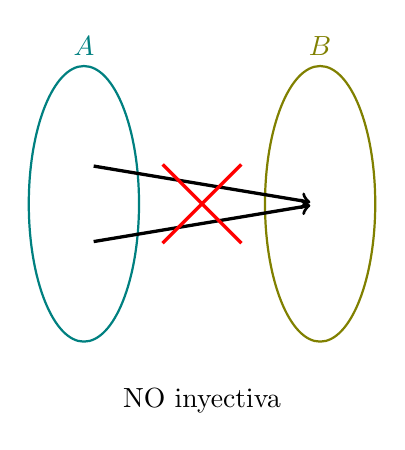
\begin{tikzpicture}
\node[color=green!50!blue] (A) at (0,4.5) {$A$};
\draw[color=green!50!blue,thick] (0.7,2.5) arc (0:-360:0.7cm and 1.75cm);
\node[color=green!50!red] (B) at (3,4.5) {$B$};
\draw[color=green!50!red,thick] (3.7,2.5) arc (0:-360:0.7cm and 1.75cm);
\node (T) at (3,2.5) {};
\node (B) at (0,2) {} edge[arrows=->,very thick] (T);
\node (C) at (0,3) {} edge[arrows=->,very thick] (T);
\draw[red,very thick] (1,3)--(2,2);
\draw[red,very thick] (1,2)--(2,3);
\node (O) at (1.5,0) {NO inyectiva};
\end{tikzpicture}
\hspace{4cm}
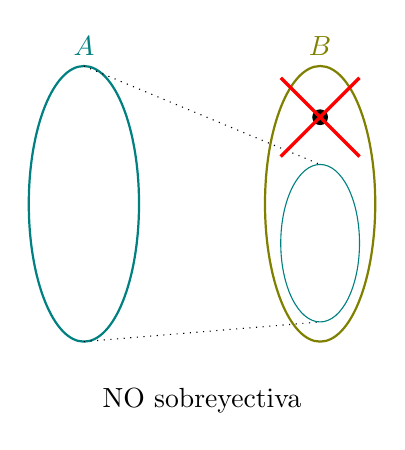
\begin{tikzpicture}
\node[color=green!50!blue] (A) at (0,4.5) {$A$};
\draw[color=green!50!blue,thick] (0.7,2.5) arc (0:-360:0.7cm and 1.75cm);
\node[color=green!50!red] (B) at (3,4.5) {$B$};
\draw[color=green!50!red,thick] (3.7,2.5) arc (0:-360:0.7cm and 1.75cm);
\draw[dotted] (0,4.25) -- (3,3);
\draw[dotted] (0,.75) -- (3,1);
\draw[color=green!50!blue] (3.5,2) arc (0:-360:0.5cm and 1cm);
\fill (3,3.6) circle (0.1);
\draw[red,very thick] (2.5,4.1)--(3.5,3.1);
\draw[red,very thick] (2.5,3.1)--(3.5,4.1);
\node (O) at (1.5,0) {NO sobreyectiva};
\end{tikzpicture}
\end{center}

Esta reflexión nos ayuda a entender conceptualmente los conceptos de inyectividad y sobreyectividad, sin embargo a la hora de analizar una función concreta, en general no podemos hacer diagramas de flechas.
El único caso en el que el uso de los diagramas de flechas podría tener utilidad práctica es el caso en que tanto el conjunto de llegada como el de partida son conjuntos finitos, y que por lo tanto se pueden estudiar por inspección exhaustiva.


\vspace{.2cm}



\begin{ejercicio}\label{reales34}
En las siguientes figuras se grafican los conjuntos $R\subset \R\times\R$ de pares $(x,y)$ que cumplen la ecuación indicada en rojo.
¿Son funciones?, ¿cuáles son inyectivas?, ¿cuáles sobreyectivas?

\begin{center}
\begin{tikzpicture}[scale=0.7,domain=-1.6:1.6]
\draw (-4,4) node {3)};
\draw[arrows=->] (-4.4,0) -- (4.4,0) node[right] {$A$};
\draw[arrows=->] (0,-4.4) -- (0,4.4) node[above] {$B$};
\foreach \pos in {-4,-3,-2,-1,1,2,3,4}
    \draw[shift={(\pos,0)}] (0,.1) -- (0,-.1) node[below] {$\pos$};
 \foreach \pos in {-4,-3,-2,-1,1,2,3,4}
    \draw[shift={(0,\pos)}] (.1,0) -- (-.1,0) node[left] {$\pos$};
 \draw[color=red]    plot (\x,\x*\x*\x)             node[right] {$b=a^3$};

\end{tikzpicture}
\begin{tikzpicture}
\draw[white] (0,0)-- (2,0);
\end{tikzpicture}
\begin{tikzpicture}[scale=0.7]
\draw (-4,4) node {4)};
\draw[arrows=->] (-4.4,0) -- (4.4,0) node[right] {$A$};
\draw[arrows=->] (0,-4.4) -- (0,4.4) node[above] {$B$};
 \foreach \pos in {-4,-3,-2,-1,1,2,3,4}
    \draw[shift={(\pos,0)}] (0,.1) -- (0,-.1) node[below] {$\pos$};
 \foreach \pos in {-4,-3,-2,-1,1,2,3,4}
    \draw[shift={(0,\pos)}] (.1,0) -- (-.1,0) node[left] {$\pos$};
 \draw[color=red]    (-1,-1)--(4,1.5)             node[above] {$2b+2=|a+1|$};
 \draw[color=red]    (-1,-1)--(-4,0.5) ;
\end{tikzpicture}
\end{center}
\end{ejercicio}

No siempre es fácil graficar funciones, como verán en Cálculo I, hay funciones muy difíciles de graficar, incluso por medio de un computador, ya que estos cometen errores de aproximación, que a veces ocultan comportamientos relevantes.
Por lo tanto, la herramienta que usaremos para estudiar funciones serán las \emph{ecuaciones}.

\vspace{.2cm}

\begin{ejemplo}
  Analicemos los conjuntos de los Ejercicios~\ref{reales12} y~\ref{reales34}.
\begin{enumerate}
\item[2)] $R|_{\R\setminus\{0\}}:\R\setminus\{0\}\rightarrow \R$, definida por $ R|_{\R\setminus\{0\}}(a)=\frac{1}{a}-3$.

Ya vimos que esta sí es una función, indaguemos el conjunto pre-imagen de un elemento $b$ aribitrario en su conjunto de llegada $\R$.
\begin{eqnarray*}
R|_{\R\setminus\{0\}}^{-1}(b)&=&\{ a\in {\R\setminus\{0\}}\ :\ R|_{\R\setminus\{0\}}(a)=b\}\\
&=&\{ a\in {\R\setminus\{0\}}\ :\ \frac{1}{a}-3=b\}\\
&=&\{ a\in {\R\setminus\{0\}}\ :\ 1=a(b+3)\}\\
&=&\{ a\in {\R\setminus\{0\}}\ :\ a=\frac{1}{b+3}\wedge b+3\not = 0\}\\
&=&\{ a\in {\R\setminus\{0\}}\ :\ a=\frac{1}{b+3}\wedge b\not = -3\}\\
&=&\left\{ \begin{array}{cl} \left\{\frac{1}{b+3}\right\} & \textrm{si } b\not = -3\\ \phi & \textrm{si } b=-3\end{array}\right.
\end{eqnarray*}
De acá obtenemos que la función no es sobreyectiva, pues hay elementos del conjunto de llegada que tienen pre-imagen vacía.
Por otra parte sí es inyectiva ya que las pre-imágenes tienen a lo más 1 elemento.
 \item[3)] $R=\{ (a,b)\in\R\times\R\ :\ b=a^3\}$

    No es difícil ver que $R(a)=a^3$, todo elemento de $A=\R$ tiene una única imagen en $B=\R$, por lo tanto ¡esta sí es una función!

    Analicemos ahora su inyectividad y sobreyectividad.
    Para ello debemos calcular el conjunto de pre-imagen de un elemento $b\in B$ arbitrario.
    \begin{eqnarray*}
      R^{-1}(b)&=& \{a\in A\ :\ b=a^3\}\\
      &=& \{\sqrt[3]{b}\}
    \end{eqnarray*}
    Vemos que este conjunto siempre tiene un único elemento: $|R^{-1}(b)|=|\{\sqrt[3]{a}\}|=1$.
    Lo cual nos dice que esta función es tanto inyectiva como sobreyectiva.
    Esto gracias a que la raíz cúbica está siempre definida en los reales, y es la única solución de la ecuación $b=x^3$.

    \item[4)] $R=\{ (a,b)\in\R\times\R\ :\ 2b+2=|a+1|\}$
    
    Acá tampoco es difícil despejar $b$ para obtener que $R(a)=\frac{|a+1|-2}{2}$, por lo tanto también estamos frente a una función.
    
    Respecto a su inyectividad, su gráfico nos muestra que adolece del mismo problema que $C$: hay elementos del eje $Y$ que tienen dos pre-imágenes y hay elementos que no tienen ninguna, con lo cual no es ni inyectiva ni sobreyectiva.
    
    Para calcular el conjunto pre-imagen en cada caso podemos proceder de manera analítica.   
     \begin{eqnarray*}
      R^{-1}(b)&=& \{a\in A\ :\ b=\frac{|a+1|-2}{2}\}\\
      &=& \{a\in A\ :\ 2b+2=|a+1|\}\\
    \end{eqnarray*}   
    Llegado a este punto, no queda más que trabajar por casos, puesto que es así como está definida la función módulo:
  $$|x|=\left\{\begin{array}{rl} x&\textrm{si } x\ge 0\\ -x &\textrm{si }x<0\end{array}\right.$$
    Esto significa que tenemos dos ecuaciones diferentes dependiendo de en qué rango esté potencialmente $a$.
    Podemos entonces trabajar la ecuación como sigue.
     \begin{eqnarray*}
       2b+2=|a+1|&\Leftrightarrow& [a+1\ge 0\wedge 2b+2=a+1]\vee[a+1<0\wedge 2b+2=-a-1]\\
       &\Leftrightarrow& [a\ge -1\wedge a=2b+1]\vee[a<-1\wedge a=-2b-3]\\
       &\Leftrightarrow& [2b+1\ge -1\wedge a=2b+1]\vee[-2b-3<-1\wedge a=-2b-3]\\
       &\Leftrightarrow& [b\ge -1\wedge a=2b+1]\vee[b>-1\wedge a=-2b-3]
     \end{eqnarray*} 
Como en ambos casos se debe cumplir que $b\ge -1$ vemos que esta es una condición necesaria y suficiente para la existencia de pre-imagen.
Por otra parte, cuando esto se cumple, $a$ puede tomar dos valores diferentes, así,  
\begin{eqnarray*}
      R^{-1}(b)&=& \left\{\begin{array}{ll}
      \{2b+1, -2b-3\} &\textrm{si } b> -1\\
      \{2b+1\} &\textrm{si } b= -1\\
      \phi &\textrm{si } b< -1
      \end{array}\right.
    \end{eqnarray*}     
  \end{enumerate}
\end{ejemplo}

\hspace{.5cm}

\begin{defn}
Dada una función  $R:A\rightarrow B$, se define el \emph{recorrido} de $R$  como el conjunto de puntos en $B$ que tienen al menos una pre-imagen:
\begin{eqnarray*}
Rec(R)&=&\{ b\in B\ :\ |R^{-1}(b)|\ge 1\}\\
&=&\{ b\in B\ :\ R^{-1}(b)\neq \phi\}\\
&=&\{ b\in B\ :\ \exists a\in A, R(a)=b\}\\
&=&\{ R(a)\ :\ a\in A\}.
\end{eqnarray*}
\end{defn}
Según esta definición, y dado los análisis hechos más arriba, podemos calcular explícitamente el recorrido de la función $C$.
$$Rec(C)=[-2,\infty)$$
Si no hubiésemos hecho el análisis previo, habríamos podido llegar al mismo resultado mediante el siguiente cálculo.
\begin{eqnarray*}
Rec(C)&=&\{ y\in B\ :\ \exists x\in A, C(x)=y\}\\
&=&\{ y\in B\ :\ \exists x\in A, x^4-2=y\}
\end{eqnarray*}
Trabajamos la última ecuación que define el conjunto; debemos manejarla con mucho cuidado, transformándola de manera de obtener siempre ecuaciones equivalentes, como sigue.
\begin{eqnarray*}
\exists x\in A, x^4-2=y&\Leftrightarrow& \exists x\in A, x^4=y+2\\
&\Leftrightarrow& \exists x\in A, x=\sqrt[4]{y+2}\\
&\Leftrightarrow& y+2\ge 0\\
&\Leftrightarrow& y\ge -2\\
\end{eqnarray*}
\vspace{-1cm}
Así,
\begin{eqnarray*}
Rec(C)&=&\{ y\in B\ :\ y\ge -2\}\\
&=&[-2,\infty)
\end{eqnarray*}
Dada la definición de recorrido podemos caracterizar la sobreyectividad de una función como la propiedad de tener recorrido igual a su conjunto de llegada $B$.

\hspace{.2cm}

\begin{thm}
Dada una función  $R:A\rightarrow B$, se cumple que
$$R \textrm{ es sobreyectiva }\quad \Longleftrightarrow\quad Rec(R)=B.$$
\end{thm}
El hecho que $Rec(C)=[-2,\infty)\not=\R$, es una evidencia adicional de la no sobreyectividad de $C$.

\hspace{.5cm}

\begin{defn}
Una función  $R:A\rightarrow B$ se dice \emph{biyectiva} si es inyectiva y sobreyectiva al mismo tiempo, es decir si
$$\textrm{para todo } b\in B \textrm{ se cumple que }|R^{-1}(b)|= 1.$$
\end{defn}

De los ejemplos anteriores, solo el ejemplo 3) de la función $R(a)=a^3$ es biyectiva.

Cuando una función es biyectiva, tenemos que cada elemento tiene exactamente una pre-imágen, por lo tanto podemos definir una función que a cada elemento del espacio de llegada le asocia su pre-imágen, tal será su \emph{función inversa}. 

Esta operación se puede visualizar muy buen cuando se mira la función como sub conjunto del producto cartesiano: Si $C\subseteq A\times B$ es una función biyectiva, entonces el conjunto:
$$ C^{-1}=\{(b,a)\ :\ (a,b)\in C\}$$
será también una función, y será la función inversa de $C$.

\hspace{.2cm}


\begin{ejemplo}
En la función 3) del Ejercicio~\ref{reales34}, que es biyectiva, podemos definir la función $R^{-1}: B\rightarrow A$ por $R^{-1}(b)=\sqrt[3]{b}$, graficada en azul en la figura.
Vemos que $R^{-1}$ es el reflejo especular de $R$ respecto a la recta diagonal en verde, que corresponde a la ecuación $a=b$.

\begin{center}
\begin{tikzpicture}[domain=-1.6:1.6]
\draw[arrows=->] (-4.4,0) -- (4.4,0) node[right] {$A$};
\draw[arrows=->] (0,-4.4) -- (0,4.4) node[above] {$B$};
\foreach \pos in {-4,-3,-2,-1,1,2,3,4}
    \draw[shift={(\pos,0)}] (0,.1) -- (0,-.1) node[below] {$\pos$};
 \foreach \pos in {-4,-3,-2,-1,1,2,3,4}
    \draw[shift={(0,\pos)}] (.1,0) -- (-.1,0) node[left] {$\pos$};
 \draw[color=red]    plot (\x,\x*\x*\x)             node[right] {$R(a)=a^3$};
 \draw[color=blue]    plot (\x*\x*\x,\x)             node[right] {$R^{-1}(b)=\sqrt[3]{b}$};
\draw[green,very thick,dashed] (-4,-4) --(4,4);
\end{tikzpicture}
\end{center}
\end{ejemplo}


\subsection{Operaciones entre funciones}

Hay algunas funciones destacadas que se pueden definir siempre.

{\bf Función identidad.} Dado un conjunto $A$, la función identidad de $A$ se denota por $id_A$ y se define como $id_A:A\rightarrow A$, donde para todo $a\in A, id_A(a)=a$, es decir, es una función que no modifica al objeto, y es claramente funcional.
En este caso $Rec(id_A)=A$, $id_A$ es biyectiva y $id_A^{-1}=id_A$.

{\bf Función constante.} Se dice que una función $f:A\rightarrow B$ es constante si se cumple que para todo $x,y\in A, f(x)=f(y)$; es decir, $f$ lleva a todos los elementos de $A$ a un solo elemento de $B$ fijo.
En este caso $|Rec(f)|=1$, la función no será ni inyectiva ni sobreyectiva, salvo en los casos triviales en que $A$ o $B$ tengan un solo elemento, respectivamente.

Estas funciones se encontrarán muy rara vez en las aplicaciones, sin embargo serán útiles en asuntos teóricos y para describir ciertos fenómenos.
Pero definamos ahora la operación más importante que se puede definir entre funciones abstractas.

Muchas veces necesitamos aplicar una transformación a un objeto y luego aplicar otra, esto se conceptualiza con la siguiente definición.

\vspace{.2cm}

\begin{defn}
Dadas dos funciones $F:A\rightarrow B$ y $G:C\rightarrow D$, decimos que $G$ se pude componer con $F$ si y solo si $B=C$, en tal caso la función compuesta $G\circ F$ va de $A$ en $D$ y queda definida como sigue.
$$G\circ F:A\rightarrow D$$
$$x\in A\rightarrow G\circ F(x)=G(F(x))$$
\end{defn}

Hacemos notar que para poder componer una función con otra es necesario que la primera tenga conjunto de llegada igual al conjunto de partida de la segunda, si no es así, no se puede definir la composición.

\vspace{.2cm}

\begin{ejemplo}
Veamos un ejemplo simple primero, consideremos la función $H$ del ejemplo~\ref{grafos}, y la función $K:\{0,1,2,3\}\rightarrow\{1,2,3\}$ definida por $K(0)=1$, $K(1)=1$, $K(2)=3$, $K(3)=3$.
Como el conjunto de llegada de $K$ coincide con el conjunto de partida de $H$ podemos componer y obtener $H\circ K$.
El el grafo se ve más claro.
Con flechas negras representamos la función $K$ y la función $H$, mientras que con flechas rojas representamos la función $H\circ K$.
\begin{center}
\begin{tikzpicture}[bend angle=10]
\node (O) at (1.5,5) {$H$};
\node[shape=rectangle,right,draw] (H) at (3,1) {$\heartsuit$};
\node[shape=rectangle,right,draw] (E) at (3,2) {$\spadesuit$};
\node[shape=rectangle,right,draw] (T) at (3,3) {$\clubsuit$};
\node[shape=rectangle,right,draw] (D) at (3,4) {$\Diamond$};
\node[shape=rectangle,left,draw] (A) at (0,1) {$1$} edge[arrows=->,very thick] (E);
\node[shape=rectangle,left,draw] (B) at (0,2) {$2$} edge[arrows=->,very thick] (D);
\node[shape=rectangle,left,draw] (C) at (0,3) {$3$} edge[arrows=->,very thick] (T);
\node (K) at (-1.5,5) {$K$};
\node[shape=rectangle,left,draw] (K0) at (-3,1) {$0$} edge[arrows=->,very thick] (A)
edge[arrows=->,very thick,red] (E);
\node[shape=rectangle,left,draw] (K1) at (-3,2) {$1$} edge[arrows=->,very thick] (A)
edge[arrows=->,very thick,red,bend right] (E);
\node[shape=rectangle,left,draw] (K2) at (-3,3) {$2$} edge[arrows=->,very thick] (C)
edge[arrows=->,very thick,red,bend right] (T);
\node[shape=rectangle,left,draw] (K3) at (-3,4) {$3$} edge[arrows=->,very thick] (C)
edge[arrows=->,very thick,red] (T);
\node[red] (HK) at (0,0) {$H\circ K$};
\end{tikzpicture}
\end{center}
\end{ejemplo}


\begin{ejemplo}\label{ca}
Veamos otro ejemplo simple, pero entre funciones numéricas.
Consideremos $c:\R\rightarrow \R$, definida por $c(x)=x^2$, y $a:\R\rightarrow \R$, definida por $a(x)=x+2$.
Podemos definir tanto $c\circ a$ como $a\circ c$ pues los conjuntos de partida y llegada de las dos funciones son todos iguales.
\begin{center}
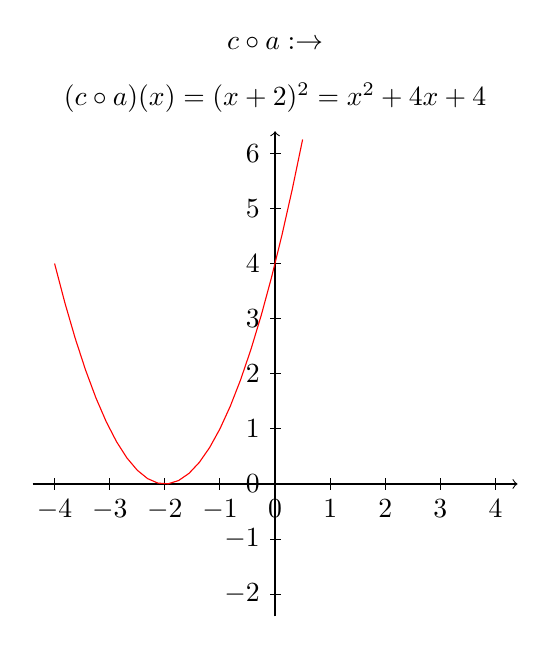
\begin{tikzpicture}[scale=0.7,domain=-4:0.5]
\node (ca) at (0,8) {$c\circ a:\R\rightarrow\R$};
\node (ca) at (0,7) {$(c\circ a)(x)=(x+2)^2=x^2+4x+4$};
\draw[arrows=->] (-4.4,0) -- (4.4,0);
\draw[arrows=->] (0,-2.4) -- (0,6.4);
 \foreach \pos in {-4,-3,-2,-1,0,1,2,3,4}
    \draw[shift={(\pos,0)}] (0,.1) -- (0,-.1) node[below] {$\pos$};
 \foreach \pos in {-2,-1,0,1,2,3,4,5,6}
    \draw[shift={(0,\pos)}] (.1,0) -- (-.1,0) node[left] {$\pos$};
 \draw[color=red]    plot (\x,\x*\x+4*\x+4) ;
\end{tikzpicture}
\begin{tikzpicture}
\draw[white] (0,0)-- (2,0);
\end{tikzpicture}
\begin{tikzpicture}[scale=0.7,domain=-2:2]
\node (ac) at (0,8) {$a\circ c:\R\rightarrow\R$};
\node (ac) at (0,7) {$(a\circ c)(x)=x^2+2$};
\draw[arrows=->] (-4.4,0) -- (4.4,0);
\draw[arrows=->] (0,-2.4) -- (0,6.4);
 \foreach \pos in {-4,-3,-2,-1,0,1,2,3,4}
    \draw[shift={(\pos,0)}] (0,.1) -- (0,-.1) node[below] {$\pos$};
 \foreach \pos in {-2,-1,0,1,2,3,4,5,6}
    \draw[shift={(0,\pos)}] (.1,0) -- (-.1,0) node[left] {$\pos$};
\draw[color=red]    plot (\x,\x*\x+2);
\end{tikzpicture}
\end{center}
\end{ejemplo}


\begin{prop}
La operación de composición de funciones es asociativa pero no conmutativa.
\end{prop}
{\bf Demostración.}
De los dos ejemplos anteriores se evidencia que la composición {\bf no es conmutativa}, en el primer ejemplo la composición $K\circ H$ ni siquiera tiene sentido. 
En el segundo ejemplo tanto $a\circ c$ como $c\circ a$ tienen sentido, pero $a\circ c\not =c\circ a$.

Veamos ahora que la asociatividad sí se cumple.
Para ello supongamos que tenemos tres funciones $R:A\rightarrow B$, $S:B\rightarrow C$, $T:C\rightarrow D$, de manera tal que es posible definir 
\begin{itemize}
\item $S\circ R:A\rightarrow C$ y $T\circ(S\circ R):A\rightarrow D$, y también
\item $T\circ S:B\rightarrow D$ y $(T\circ S)\circ R:A\rightarrow D$.
\end{itemize}
Queremos demostrar que $T\circ(S\circ R)=(T\circ S)\circ R$.
De momento tenemos al menos que sus conjuntos de partida y llegada coinciden.
Ahora debemos demostrar que toman los mismos valores, es decir, debemos demostrar que:
$$ \forall x\in A,\ (T\circ(S\circ R))(x)=((T\circ S)\circ R)(x).$$
Para demostrar esto, aplicamos la definición de composición cuidadosamente.
Tomemos antes que nada un $x$ cualquiera en $A$, así lo que demostremos será válido en todo $x$.
\begin{align*}
(T\circ(S\circ R))(x)&=T((S\circ R)(x));&\textrm{por definición de }T\circ(S\circ R)\\
&=T(S(R(x)))&\textrm{por definición de }S\circ R,
\end{align*}
por otra parte,
\begin{align*}
((T\circ S)\circ R)(x)&=(T\circ S)(R(x));&\textrm{por definición de }(T\circ S)\circ R\\
&=T(S(R(x)))&\textrm{por definición de }T\circ S.
\end{align*}
Como en ambos desarrollos se llega a lo mismo, queda claro que $(T\circ(S\circ R))(x)=((T\circ S)\circ R)(x)$.
\hfill $\Box$

Observamos que la función $id_A$ e $id_B$ actúan como neutro respecto a la composición, es decir: $id_B\circ F=F$ y $F\circ id_A=F$.
En efecto $(id_B\circ F)(x)=id_B(F(x))=F(x)$, ya que $id_B$ no modifica el valor $F(x)$.
Análogamente $(F\circ id_A)(x)=F(id_A(x))=F(x)$, ya que $id_B$ no modifica el valor $x$.

\subsection{Inversa de una función}

Podemos repasar la función inversa mediante el uso de la composición de funciones y la función identidad gracias al siguiente teorema.

\vspace{.2cm}

\begin{thm}
$F:A\rightarrow B$ es biyectiva si y solo si existe $H:B\rightarrow A$ tal que $F\circ H=id_B$ y $H\circ F=id_A$.\\
\end{thm}
{\bf Demostración.}
\begin{itemize}
\item  {\bf ($\Rightarrow$)} Cuando $F$ es biyectiva vimos que podemos definir $F^{-1}:B\rightarrow A$.
 Tomando $H=F^{-1}$ se cumple todo lo deseado ya que si $y=F(x)$, entonces $x=H(y)$, así: 
 \begin{itemize}
 \item $H(F(x))=H(y)=x=id_A(x)$ y por su parte 
 \item $F(H(y))=F(x)=y=id_B(y)$.
 \end{itemize}
 \item  {\bf ($\Leftarrow$)} En este caso asumimos que existe $H:B\rightarrow A$ tal que $F\circ H=id_B$ y $H\circ F=id_A$, debemos demostrar que entonces $F$ es biyectiva.
\begin{itemize}
\item {\bf $F$ es sobreyectiva.} Debemos demostrar que $|F^{-1}(y)|\ge 1$ para todo $y\in B$.
De $F\circ H=id_B$ sospechamos que una pre-imagen de $y$ debe ser $H(y)$, en efecto $F(H(y))=(F\circ H)(y)=id_B(y)=y$, así $F^{-1}(y)\supseteq\{H(y)\}$.
\item {\bf $F$ es inyectiva.} Debemos demostrar que  $|F^{-1}(y)|\le 1$ para todo $y\in B$, es decir que $H(y)$ es la única pre-imagen de $y$. Razonemos por contradicción, supongamos que hay otra, es decir que existe $z\in A$ tal que $z\not =H(y)$ y $F(z)=y$.

De $H\circ F=id_A$ tenemos que $(H\circ F)(z)=H(F(z))=id_A(z)=z$, sin embargo de nuestro supuesto tenemos que  $H(F(z))=H(y)\not=z$, hemos llegado a una contradicción, por lo tanto $y$ tiene una única pre-imagen y entonces $F$ es inyectiva.
\end{itemize}
\end{itemize}
\hfill $\Box$

\begin{ejemplo}
La función $a$ del ejemplo~\ref{ca} es invertible pues si tomamos $b:\R\rightarrow \R$ definida por $b(x)=x-2$, se cumple que 
\begin{itemize}
\item $a\circ b:\R\rightarrow\R$ se puede definir y $(a\circ b)(x)=a(b(x))=a(x-2)=x-2+2=x=id_\R(x)$, por su parte
\item $b\circ a:\R\rightarrow\R$ se puede definir y $(b\circ a)(x)=b(a(x))=b(x+2)=x+2-2=x=id_\R(x)$.
\end{itemize}
\end{ejemplo}


\vspace{.2cm}


\begin{thm}
Si $F:A\rightarrow B$ y $G:B\rightarrow C$ son invertibles, entonces $G\circ F$ es también invertible y $(G\circ F)^{-1}=F^{-1}\circ G^{-1}$ .
\end{thm}
{\bf Demostración.}
Si $F:A\rightarrow B$ y $G:B\rightarrow C$ son invertibles, entonces existen sus inversas $F^{-1}:B\rightarrow A$ y $G^{-1}:C\rightarrow B$, para demostrar lo que se pide basta verificar que la función $F^{-1}\circ G^{-1}$ está definida de $C$ en $A$ y cumple la definición de inversa, es decir que al componerla con $G\circ F$ por un lado y otro, resultan las correspondientes funciones identidad.

Primero vemos que $F^{-1}\circ G^{-1}$ está definida pues en efecto el conjunto de llegada de $G^{-1}$ es $B$ y el conjunto de partida de $F^{-1}$ es también $B$.
Así $F^{-1}\circ G^{-1}:C\rightarrow A$ está definida.

Veamos ahora la composición de esta con $G\circ F$.
Como hipótesis tenemos que $G\circ G^{-1}=id_C$, $G^{-1}\circ G=id_B$, $F\circ F^{-1}=id_B$, $F^{-1}\circ F=id_A$.
Usaremos también la asociatividad de la composición antes demostrada.

\begin{itemize}
\item {\bf $(G\circ F)\circ (F^{-1}\circ G^{-1})=id_C$} En efecto,
\begin{align*}
(G\circ F)\circ(F^{-1}\circ G^{-1})&=((G\circ F)\circ F^{-1})\circ G^{-1},&\textrm{por asociatividad aplicada a }G^{-1}\\
&=(G\circ (F\circ F^{-1}))\circ G^{-1},&\textrm{por asociatividad aplicada a }G\\
&=(G\circ id_B)\circ G^{-1},&\textrm{por hipótesis}\\
&=G\circ G^{-1},&\textrm{por neutralidad de } id_B\\
&=id_C,&\textrm{por hipótesis.}
\end{align*}
\item {\bf $(F^{-1}\circ G^{-1})\circ(G\circ F)=id_A$} {\em Es análogo al ítem anterior, sin embargo es un buen ejercicio y se recomienda hacerlo paso a paso.}
\end{itemize}
\hfill $\Box$

%%%%%%%%%%%%%%%%%%%%%%%%%%%%%%%%%%%%%%%%%%%%%%%%%inicio restricción y extensión%%%%%%%%%%%%%%%%

\subsection{Arreglando la composición}

Pero en algunas aplicaciones puede interesarnos componer funciones cuyo conjuntos de llegada y partida no calzan, veamos cuál es el problema en este caso.
Supongamos que tenemos $f:A\rightarrow B$ y $g:C\rightarrow D$.
Dos casos aparecen.
\begin{center}
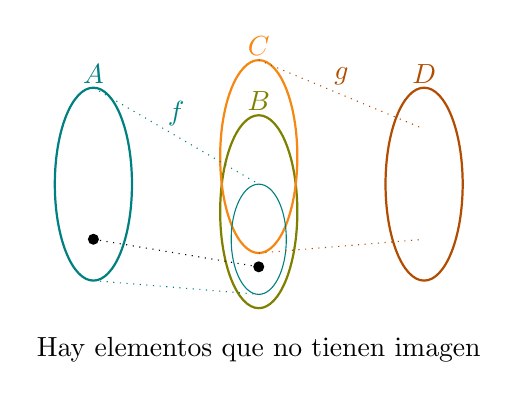
\begin{tikzpicture}[scale=.7]
\node[color=green!50!blue] (A) at (0,5) {$A$};
\draw[color=green!50!blue,thick] (0.7,3) arc (0:-360:0.7cm and 1.75cm);
\node[color=green!50!red] (B) at (3,4.5) {$B$};
\draw[color=green!50!red,thick] (3.7,2.5) arc (0:-360:0.7cm and 1.75cm);
\node[color=yellow!50!red] (B) at (3,5.5) {$C$};
\draw[color=yellow!50!red,thick] (3.7,3.5) arc (0:-360:0.7cm and 1.75cm);
\node[color=green!30!red] (B) at (6,5) {$D$};
\draw[color=green!30!red,thick] (6.7,3) arc (0:-360:0.7cm and 1.75cm);
\draw[dotted,green!50!blue] (0,4.75) -- (3,3) node[above,midway] {$f$};
\draw[dotted,green!50!blue] (0,1.25) -- (3,1);
\draw[color=green!50!blue] (3.5,2) arc (0:-360:0.5cm and 1cm);
\fill (3,1.5) circle (0.1);
\fill (0,2) circle (0.1);
\draw[dotted] (0,2) -- (3,1.5);
\draw[dotted,green!30!red] (3,5.25) -- (6,4) node[above,midway] {$g$};
\draw[dotted,green!30!red] (3,1.75) -- (6,2);

\node (O) at (3,0) {Hay elementos que no tienen imagen};
\end{tikzpicture}
\begin{tikzpicture}
\draw[white] (0,0)--(1,0);
\end{tikzpicture}
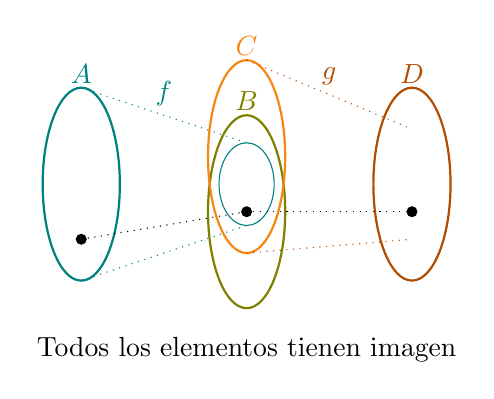
\begin{tikzpicture}[scale=.7]
\node[color=green!50!blue] (A) at (0,5) {$A$};
\draw[color=green!50!blue,thick] (0.7,3) arc (0:-360:0.7cm and 1.75cm);
\node[color=green!50!red] (B) at (3,4.5) {$B$};
\draw[color=green!50!red,thick] (3.7,2.5) arc (0:-360:0.7cm and 1.75cm);
\node[color=yellow!50!red] (C) at (3,5.5) {$C$};
\draw[color=yellow!50!red,thick] (3.7,3.5) arc (0:-360:0.7cm and 1.75cm);
\node[color=green!30!red] (D) at (6,5) {$D$};
\draw[color=green!30!red,thick] (6.7,3) arc (0:-360:0.7cm and 1.75cm);
\draw[dotted,green!50!blue] (0,4.75) -- (3,3.75) node[above,midway] {$f$};
\draw[dotted,green!50!blue] (0,1.25) -- (3,2.25);
\draw[color=green!50!blue] (3.5,3) arc (0:-360:0.5cm and .75cm);
\fill (3,2.5) circle (0.1);
\fill (0,2) circle (0.1);
\fill (6,2.5) circle (0.1);
\draw[dotted] (0,2) -- (3,2.5);
\draw[dotted] (3,2.5) -- (6,2.5);
\draw[dotted,green!30!red] (3,5.25) -- (6,4) node[above,midway] {$g$};
\draw[dotted,green!30!red] (3,1.75) -- (6,2);

\node (O) at (3,0) {Todos los elementos tienen imagen};
\end{tikzpicture}
\end{center}
El caso de la derecha no parece muy grave, la función compuesta se puede calcular, solo sería necesario redefinir el conjunto de llegada de $f$ y el conjunto de partida de $g$ de manera que fueran iguales, para lo cual lo más sencillo probablemente es tomar ambos como $B\cap C$.
Esto funciona ya que $Rec(f)\subseteq B\cap C$.

Por ejemplo, para formalizar esta idea, podemos definir las funciones $\tilde{f}:A\rightarrow B\cap C$, como $\tilde{f}(x)=f(x)$ para todo $x\in A$, y $\tilde{g}:B\cap C\rightarrow D$ como $\tilde{g}(x)=g(x)$ para todo $x\in B\cap C$.
Con esto la función $\tilde{g}\circ\tilde{f}:A\rightarrow D$ se puede definir y resulta, como es de esperarse, $(\tilde{g}\circ\tilde{f}(x))=g(f(x))$, para todo $x\in A$.

El caso de la izquierda, sin embargo, es más complicado pues si restringiéramos el conjunto de llegada de $f$, quedarían elementos sin imagen, y $f$ dejaría de ser una función.
En este caso será necesario achicar también el conjunto $A$, eliminando todos esos elementos que quedan sin imagen.

En general, dadas dos funciones cualesquiera $f:Dom(f)\subseteq A\rightarrow B$ y $g:Dom(g)\subseteq C\rightarrow D$, podemos definir:
$$ Dom(g\circ f)=\{x\in A\ :\ f(x)\in Dom(g)\},$$
con lo cual se puede definir la función compuesta: $(g\circ f):Dom(f\circ g)\subset A\rightarrow D$, como siempre: $(g\circ f)(x)=g(f(x))$.

\vspace{.2cm}

\begin{ejemplo}
Tomemos $f:Dom(f)\subseteq \R\rightarrow \R$ y $g:Dom(g)\subseteq \R\rightarrow \R$ definidas por $f(x)=x^2-1$, y $g(t)=log(x+3)$, respectivamente.
Entonces,
\begin{eqnarray*}
Dom(g\circ f)&=&\{x\in \R\ :\ f(x)\in Dom(g)\}\\
&=&\{x\in \R\ :\ x^2-1\in (-3,\infty)\}\\
&=&\{x\in \R\ :\ x^2-1>3\}\\
&=&\{x\in \R\ :\ x^2>4\}=(-\infty,-2)\cup(2,\infty)
\end{eqnarray*}
\end{ejemplo}

\section{Funciones Reales}

Las operaciones y conceptos definidos más arriba son válidos para funciones en cualquier par de conjuntos.
Pero nosotros trabajaremos frecuentemente con funciones entre números, reales, naturales, enteros o racionales, pero números al fin.
En esos casos podemos definir conceptos adicionales y operaciones adicionales.

%%%%%%%%%%%


\subsection{Paridad}
Otra de las propiedades bonitas que se pueden estudiar de una función es la ``paridad'', la cual no tiene nada que ver con la paridad de los números enteros.

\vspace{.2cm}

\begin{defn}
Dada una funci\'on $f : A\subseteq \R \To \R$ decimos que su conjunto es \emph{simétrico} respecto a $0$ si cumple que $\forall\,x \in A,\  -x \in A$.

Si $f$ tiene un conjunto de partida simétrico respecto a $0$, entonces decimos que  \emph{$f$ es
 par} si y solo si 
\[
	\forall\, x \in A\;:\; f(x) = f(-x),
\]
y decimos que  \emph{$f$ es impar}  si y solo si
\[
	\forall\, x \in A\;:\; f(x) = -f(-x).
\]
\end{defn}

\begin{ejemplo}
	Note que
	\begin{enumerate}
		\item $R(x) = x^3$ es impar pues
			\[
				R(-x) = (-x)^3 = (-1)^3x^3=(-1)x^3=-x^3= -R(x).
			\]
		\item $C(x) = x^4-2$ es par, en efecto,
			\[
				C(-x) = (-x)^4-2 = (-1)^4x^4-2=x^4-2 = C(x).
			\]
	\end{enumerate}
	
\begin{center}
\begin{tikzpicture}[scale=0.7,domain=-1.6:1.6]
\draw[white,dashed] (0,-6) --(0,6);
\draw[arrows=->] (-4.4,0) -- (4.4,0) node[right] {$\R$};
\draw[arrows=->] (0,-4.4) -- (0,4.4) node[above] {$\R$};
\foreach \pos in {-4,-3,-2,-1,1,2,3,4}
    \draw[shift={(\pos,0)}] (0,.1) -- (0,-.1) node[below] {$\pos$};
 \foreach \pos in {-4,-3,-2,-1,1,2,3,4}
    \draw[shift={(0,\pos)}] (.1,0) -- (-.1,0) node[left] {$\pos$};
 \draw[color=red]    plot (\x,\x*\x*\x)             node[right] {$R(a)=a^3$};
 \draw[green,very thick,arrows=->] (95:1.5) arc[start angle=95, end angle=175, radius=1.5];
\end{tikzpicture}
\begin{tikzpicture}
\draw[white] (0,0)--(1,0);
\end{tikzpicture}
\begin{tikzpicture}[scale=0.7,domain=-1.6:1.6]
\draw[arrows=->] (-4.2,0) -- (4.2,0) node[right] {$\R$};
\draw[arrows=->] (0,-4.2) -- (0,4.2) node[above] {$\R$};
 \foreach \pos in {-4,-3,-2,-1,1,2,3,4}
    \draw[shift={(\pos,0)}] (0,.1) -- (0,-.1) node[below] {$\pos$};
 \foreach \pos in {-4,-3,-2,-1,1,2,3,4}
    \draw[shift={(0,\pos)}] (.1,0) -- (-.1,0) node[left] {$\pos$};
 \draw[color=red]    plot (\x,\x*\x*\x*\x-2)             node[right] {$C(x)=x^4-2$};
\draw[green,very thick,dashed] (0,-6) --(0,6);
\end{tikzpicture}\end{center}


\end{ejemplo}

Note que una funci\'on puede no ser ni par ni impar, por ejemplo,
$f(x) = x+1$ no es ni par ni impar, veamos:
\[
	f(-x) = -x+1 \ne f(x),\quad  -f(x)=-(x+1)=-x-1\neq f(-x) = -x+1.
\]

\subsection{Periodo}

Algunas funciones con dominio en $\R$ pueden ser periódicas, representan movimientos repetitivos, fenómenos repetitivos, como por ejemplo las oscilaciones o las estaciones del año.

\vspace{.2cm}

\begin{defn}
Dada una funci\'on $f :  \R \To \R$ y un número positivo $p$, decimos que  \emph{$f$ es
 periódica de periodo $p$} si y solo si se cumple
 $$ \forall x\in\R, f(x+p)=f(x).$$
\end{defn}

Una función periódica tendrá un gráfico que es repetitivo, todo lo que observemos para $x\in[0,p)$, lo veremos repetido en $[p,2p)$ y en $[2p,3p)$ etcétera.
Esta propiedad se ilustra muy bien mediante las funciones trigonométricas, que veremos más adelante.

\subsection{Operaciones entre funciones reales}

Si se trata de funciones en los reales, también podemos definir las siguientes operaciones.
\begin{defn}
	Dadas las funciones $f : A\subseteq \R \To \R$ y $g: B \subseteq \R \To \R$, tales que $A\cap B\not =\phi$ y un escalar $\lambda \in \R$, se definen:
	las siguientes \emph{operaciones entre $f$ y $g$}:
	\begin{enumerate}
		\item Ponderación: $\lambda\,f: A \To \R$ por $(\lambda\,f)(x) = \lambda\,f(x)$,
		\item Suma: $f+ g : A \cap B \To \R$ por $(f+ g)(x) = f(x)+ g(x)$,
		\item Multiplicación: $fg: A \cap B \To \R$ por $(fg)(x) = f(x)g(x)$,
		\item Cuociente: Si $(A \cap B) \setminus \{x \in B\;:\; g(x) = 0\}\not = \phi$, entonces definimos 
		$$\dfrac f g: (A \cap B) \setminus \{x \in B\;:\; g(x) = 0\} \To \R,\textrm{ por}$$
			$$\left(\dfrac f g\right)(x) = \dfrac{f(x)}{g(x)}.$$
	\end{enumerate}
\end{defn}

\vspace{1cm}

\begin{ejemplo}
		Sean\footnote{notar que estas funciones son composición, $f$, de una recta con el módulo, y, $g$, de una recta con la raíz cuadrada, cada una restringuda además a un conjunto de partida dado.} $f: [-8,\infty[ \To \R$ y $g: ]-\infty,1] \To \R$ tales que
		\[
			f(x) = |x+8|,\qquad g(x) = \sqrt{1-x}.
		\]
		Entonces,
		\begin{enumerate}
			\item $2f : [-8,\infty] \To \R$ con $(2f)(x) = 2f(x) = 2|x+8|$, la ponderación no cambia el conjunto de partida de la función que pondera.
		\end{enumerate}
Para calcular las otras 3 operaciones, debemos calcular la intersección de los conjuntos de partida de $f$ y $g$: $[-8,\infty[\ \cap\  ]-\infty,1]=[-8,1]$.
Entonces,
		\begin{enumerate} \setcounter{enumi}{1}
			\item $f+g: [-8,\,1] \To \R$ con $(f+g)(x) = f(x) + g(x) = |x+8| + \sqrt{1-x}$;
			\item $fg: [-8,\,1] \To \R$ con $(fg)(x) = f(x)g(x) = |x+8|\sqrt{1-x}$;
		\end{enumerate}
Finalmente, para calcular el cuociente debemos identificar los puntos donde se anula $g$: 
$$\{x \in ]-\infty,1]\;:\; g(x) = 0\}=\{x \in ]-\infty,1]\;:\; \sqrt{1-x} = 0\}=\{x \in ]-\infty,1]\;:\; 1-x = 0\}=\{1\},$$
a partir de esto, el conjunto de partida de la función $\frac{f}{g}$ será $ [-8,\,1]\setminus\{1\}= [-8,\,1[$.
Entonces,
		\begin{enumerate} \setcounter{enumi}{3}
			\item $\frac f g: [-8,\,1[ \To \R$ con $(\frac f g)(x) = \frac {f(x)}{g(x)} = \frac{|x+8|}{\sqrt{1-x}}$.
		\end{enumerate}
\end{ejemplo}

Considerar estas operaciones será muy útil cuando ya conozcamos propiedades de algunas funciones, pues a veces estas propiedades serán heredadas por la resultante o al menos habrá alguna relación que se pueda deducir. 
Entonces, al ver la fórmula de una función, puede ser interesante escribirla como la operación de funciones más simples.

\begin{ejercicio}
Escriba la siguiente función como composición de funciones.
$$ h(x)=x^3+\sqrt{\left(\frac{1}{x}\right)}$$
Hay muchas maneras de hacer esto, por ejemplo consideremos $P(x)=x^3$, $id$ la función identidad, $r$ la función raíz cuadrada, y $c_1$ la función constante igual 1, entonces podemos ver que:
$$h=P+\left(r\circ\left(\frac{c_1}{id}\right)\right).$$
\end{ejercicio}

\vspace{.2cm}

\begin{prop}
Se cumplen las siguientes propiedades.
\begin{enumerate}
	\item Si $f: A\subseteq \R \To \R$ es impar y $0\in A$, entonces $f(0)=0$
	\item La única función que es par e impar al mismo tiempo es la función constante igual a 0.
	\item Si $f$ es par, entonces $f$ no es inyectiva.
	\item El gr\'afico de una funci\'on par es sim\'etrico con
		respecto al eje Y.
	\item La suma de funciones pares es par.
	\item La suma de funciones impares es impar.
	\item Todas las funciones reales sobre un conjunto de partida simétrico son suma de una función par más una impar.
	\item La multiplicación de funciones pares es par.
	\item La multiplicación de funciones impares es par.
	\item La multiplicación de una función par con una impar es impar.
	\item La composición de funciones pares es par.
	\item La composición de funciones impares es impar.
	\item La composición de una función par con una impar es par, independientemente del orden en que se realice la composición.	
	\item La función identidad es impar.
	\item Las funciones constantes son pares.
\end{enumerate}
\end{prop}

 
 Dejamos la demostración de estas propiedades como ejercicio.



%%%%%%%%%%%%%%%%%%%%%%%%%%%%%%%%%%%%%%%%%%%%fin rescricción y extensión%%%%%%%%%%%%%%
\subsection{Funciones potencia}

Las funciones ``potencia'' son particularmente importantes en muchos modelos de ciencias naturales, además de ser una de las clases más sencillas de funciones.
llamamos función ``potencia'' a las funciones $P:\R\rightarrow\R$, definidas por $P(x)=x^n$, donde $n\in\N\setminus\{0\}$ es un natural fijo no nulo.
En esta clase están la función cuadrática, la cúbica y la función identidad: $x^2$, $x^3$ y $x$.


\vspace{.2cm}


\begin{prop}
Dado $n\in\N$ se tiene que la función  $P:\R\rightarrow\R$, definida por $P(x)=x^n$ tiene las siguientes propiedades.
\begin{itemize}
\item Si $n$ es par: 
\begin{enumerate}
\item $P$ es par;
\item $P$ no es ni inyectiva;
\item $P$ no es sobreyectiva y $Rec(P)=[0,\infty)$;
\item $P|[0,\infty):[0,\infty)\rightarrow[0,\infty)$ es biyectiva y su inversa es $P|[0,\infty)^{-1}:[0,\infty)\rightarrow[0,\infty)$ definida por $$P^{-1}(x)=\sqrt[n]{x}.$$
\end{enumerate}
\item Si $n$ es impar:
\begin{enumerate}\setcounter{enumi}{4}
\item $P$ es impar;
\item $P$ es biyectiva y su inversa es $P^{-1}:\R\rightarrow \R$ definida por $P^{-1}(x)=\sqrt[n]{x}$.
\end{enumerate}
\end{itemize}
\end{prop}

La raíz $n$-ésima se escribe igualmente por $\sqrt[n]{x}=x^{\frac{1}{n}}$, lo cual proviene del hecho que $$(x^n)^{\frac{1}{n}}=x^{\frac{n}{n}}=x^1=x.$$

Esto abre la puerta para definir las potencias racionales, pero esto sólo podremos hacerlo como funciones de $[0,\infty)$ en $[0,\infty)$: dado un racional positivo $r=\frac{m}{n}$, se define la función potencia de exponente $r$ por $P(x)=x^{\frac{m}{n}}=(x^m)^{\frac{1}{n}}=\sqrt[n]{x^n}$, la cual se interpreta como la composición de $\sqrt[n]{x}$ con $x^m$.

\vspace{.2cm}


\begin{prop}
Dado $r=\frac{m}{n}$, con $n,m\in \N$ se tiene que la función potencia racional $P:[0,\infty)\rightarrow[0,\infty)$, definida por $P(x)=x^r$ tiene las siguientes propiedades.

\begin{enumerate}
\item $P$ es biyectiva y su inversa es $P^{-1}:[0,\infty)\rightarrow[0,\infty)$ definida por $P^{-1}(x)=x^{\frac{1}{r}}=x^{\frac{n}{m}}$;
\item $P(0)=0$;  $P(1)=1$.
\end{enumerate}
\end{prop}

Podemos definir también potencias negativas, notando que $y^{-1}=\frac{1}{y}$, así, dado un racional positivo $r=\frac{m}{n}$ definimos $P(x)=x^{-\frac{n}{m}}=\frac{1}{x^{\frac{n}{m}}}$.
Notamos que tal función no puede ser evaluada en $x=0$, entonces su dominio y su recorrido es $(0,\infty)$.

\vspace{.2cm}


\begin{prop}
Dado $r=\frac{m}{n}$, con $n,m\in \N$ se tiene que la función potencia racional negativa $P:(0,\infty)\rightarrow(0,\infty)$, definida por $P(x)=x^{-r}$ tiene las siguientes propiedades.

\begin{enumerate}
\item $P$ es biyectiva y su inversa es $P^{-1}:(0,\infty)\rightarrow(0,\infty)$ definida por $$P^{-1}(x)=x^{-\frac{1}{r}}=\frac{1}{x^{\frac{n}{m}}}=\left(\frac{1}{x}\right)^{\frac{n}{m}};$$
\item $P(1)=1$.
\end{enumerate}
\end{prop}


En cálculo verán que si $\alpha \in\R\setminus\{0\}$, de todas formas es posible definir la función $P(x)=x^{\alpha}$, en $(0,\infty)$ y tendrá propiedades similares.

Sin embargo cuando queramos definir una función potencia con conjunto de partida igual a $\R$, nos limitaremos solo a las potencias enteras.

\vspace{.2cm}


\begin{ejemplo}
Más que un ejemplo, creo que es interesante ver un gráfico de esta familia de funciones.
El Cálculo I verán otras fuertísimas propiedades de éstas funciones, su gráfico no engaña, son funciones muy regulares.
\begin{center}
\begin{tikzpicture}[]
\draw[arrows=->] (-4.4,0) -- (4.4,0) node[below] {$\R$};
\draw[arrows=->] (0,-4.4) -- (0,4.4) node[left] {$\R$};
\foreach \pos in {-4,-3,-2,-1,0,1,2,3,4}
    \draw[shift={(\pos,0)}] (0,.1) -- (0,-.1) node[below] {$\pos$};
\foreach \pos in {-4,-3,-2,-1,0,1,2,3,4}
    \draw[shift={(0,\pos)}] (.1,0) -- (-.1,0) node[left] {$\pos$};
\draw[color=red,domain=0:3]    plot (\x,\x^1.3)             node[right] {$x^{1.3}$};
\draw[color=orange,domain=0:4]    plot (\x,\x^0.5)             node[right] {$x^{0.5}$};
\draw[color=green,domain=-4:4]    plot (\x,\x)             node[right] {$x$};
\draw[color=cyan,domain=.06:4]    plot (\x,1/\x^.5)             node[right] {$x^{-0.5}$};
\draw[color=blue,domain=.35:4]    plot (\x,1/\x^1.3)             node[right] {$x^{-1.3}$};
\end{tikzpicture}
\end{center}
\end{ejemplo}

Cuando el exponente es 1, la función se dice \emph{lineal}, las funciones lineales son muy importantes. Son las únicas que se pueden calcular usando proporciones (regla de tres).

Finalmente, ya lo hemos hecho antes, pero no está de más recordarlo, podemos combinar funciones definiendo que dominen en tramos disjuntos: tendremos entonces las funciones definidas por tramos, en que hay una fórmula diferente que vale en cada tramo.


\vspace{.2cm}



	%%%%%%%%%%%%%%%%%%%%%%%%%%%%%%%%%%%%%%%%%%%%%%
\begin{ejemplo}
	A veces es necesario definir una funci\'on por tramos. Consideremos, por ejemplo, la funci\'on que
	describe el pago de impuestos en Chile. Ella debe ser tal que: si $x$ es la renta imponible mensual de
	una persona, entonces la cantidad $s(x)$ a pagar por impuesto \'unico de segunda categor\'{\i}a es:
	\begin{align*}
		s(x) = 
		\begin{cases}
			0 & 0 \le x < 13.5 \mbox{UTM},\\
			0.05(x-13,5) & 13.5 \mbox{UTM} \le x < 30 \mbox{UTM},\\
			0,825+0.10(x-30) & 30 \mbox{UTM} \le x < 50 \mbox{UTM},\\
			2,825+0.15(x-50) & 50 \mbox{UTM} \le x < 70 \mbox{UTM},\\
			5,825+0.25(x-70) & 70 \mbox{UTM} \le x < 90 \mbox{UTM},\\
			10,825+0.32(x-90) & 90 \mbox{UTM} \le x < 120 \mbox{UTM},\\
			20,425+0.37(x-120) & 120 \mbox{UTM} \le x < 150 \mbox{UTM},\\
			31,525+0.4(x-150) & x \ge 150 \mbox{UTM}.
		\end{cases}
	\end{align*}
	donde $UTM=\$69{.}265$ en la fecha en que este apunte se editó.
	El gr\'afico de esta función es como se muestra en la figura siguiente.
	
	\begin{figure}[ht]
		\begin{center}
			\begin{tikzpicture}[scale=0.9]
				\draw[arrows=->] (0,0) -- (16.2,0) node[below] {UTM};
				\draw[arrows=->] (0,0) -- (0,5.2) node[above] {$UTM$};
				 \foreach \pos in {0,50,100,150}
				    \draw[shift={(\pos/10,0)}] (0,.1) -- (0,-.1) node[below] {$\pos$};
				 \foreach \pos in {0,20,40}
				    \draw[shift={(0,\pos/10)}] (.1,0) -- (-.1,0) node[left] {$\pos$};
				 \draw[color=red,very thick] (0,0)--(1.35,0)
				 --(3,0.825/10)
				 --(5,2.825/10)
				 --(7,5.825/10)
				 --(9,10.825/10)
				 --(12,20.425/10)
				 --(15,31.525/10)
				 --(16,35.525/10);
			\end{tikzpicture}
		\end{center}
	\end{figure}
\end{ejemplo}


\subsection{Función exponencial y logaritmo}

En la sección anterior el exponente estaba fijo y la variable era la base de la potencia, ¿qué pasa si lo hacemos al revés? es decir, si la variable es el exponente y dejamos la base fija.
Como vimos antes, si queremos elevar a un exponente cualquiera, más vale que la base sea positiva, definiremos entonces la familia de las funciones \emph{exponenciales} como sigue.

\begin{defn}
Dado $b \in \R^+\setminus\{1\}$, definimos la \emph{función exponencial con base $b$} como 
$$\exp_b: \R \To \R^+,$$
$$\exp_b(x) = b^x.$$
\end{defn}

Si bien no hay problema en definir la función $\exp_1(x)=1^x=1$, no lo hacemos, pues esa función en más simple concebirla como la función constante igual a 1, tendrá un comportamiento radicalmente distinto al de las funciones exponenciales, por lo tanto es más sano quitarla de la familia.

\begin{prop}
Dado $b \in \R^+\setminus\{1\}$, la función $\exp_b$ es biyectiva, y además cumple:
\begin{itemize}
\item $\forall x\in\R,\ \exp_{1/b}(x)=\exp_b(-x)$,
\item $\exp_b(0)=1$, y
\item $exp_b(1)=b$.
\end{itemize}
\end{prop}

Son funciones muy regulares, que aparecen en muchos modelos, y en Cálculo I verán algunas de sus propiedades más importantes, como es la ``monotonía'' y su rápido crecimiento o decrecimiento, sin embargo dejaremos esos contenidos a esa otra asignatura pues requieren de herramientas que no competen a nuestro ramo.
Veamos de todas formas algunos gráficos de funciones de la familia exponencial.


\begin{center}
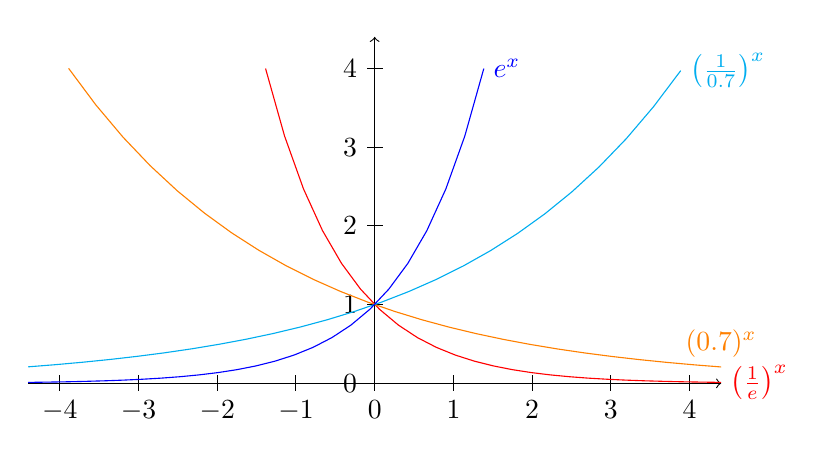
\begin{tikzpicture}[]
\draw[arrows=->] (-4.4,0) -- (4.4,0) node[below] {$\R$};
\draw[arrows=->] (0,0) -- (0,4.4) node[left] {$\R$};
\foreach \pos in {-4,-3,-2,-1,0,1,2,3,4}
    \draw[shift={(\pos,0)}] (0,.1) -- (0,-.1) node[below] {$\pos$};
\foreach \pos in {0,1,2,3,4}
    \draw[shift={(0,\pos)}] (.1,0) -- (-.1,0) node[left] {$\pos$};
\draw[color=red,domain=-1.386:4.4]    plot (\x,0.36789^\x)             node[right] {$\left(\frac{1}{e}\right)^x$};
\draw[color=orange,domain=-3.887:4.4]    plot (\x,0.7^\x)             node[above] {$(0.7)^x$};
\draw[color=cyan,domain=-4.4:3.887]    plot (\x,1.426^\x)             node[right] {$\left(\frac{1}{0.7}\right)^x$};
\draw[color=blue,domain=-4.4:1.386]    plot (\x,e^\x)             node[right] {$e^x$};
\end{tikzpicture}
\end{center}

En esta figura usamos un número particular, denotado por $e$, conocido como la \emph{constante de Euler}, el cual es un irracional, aproximado a $e\sim 2,718$, que tiene una importancia enorme en el cálculo gracias a sus sorprendentes propiedades.
La constante de Euler es una de las bases más usadas en los modelos exponenciales, junto con la base 10 y la base 2.


Recordamos aquí algunas de las propiedades de la exponenciación pues nos serán muy útiles.

\begin{multicols}{2}
\begin{enumerate}
\item $\forall b \in \R^+,\ b^1=b\wedge b^0=1$
\item $\forall b \in \R^+,\ \forall u,v\in\R,\  b^{u+v}=b^ub^v$
\item $\forall b \in \R^+,\ \forall u,v\in\R,\  (b^u)^v=b^{vu}$
\item $\forall b \in \R^+,\ \forall u\in\R,\  b^{-u}=\left(\frac{1}{b}\right)^u$
\end{enumerate}
\end{multicols}

Dado que las funciones exponenciales son invertibles, existe su inversa, la cual es llamada \emph{función logaritmo}.

\begin{defn} 
Dado $b \in \R^+\setminus\{1\}$, se define la función \emph{logaritmo en base $b$} por $\log_b := \exp_b^{-1}$, es decir,
$$\log_b : \R^+ \To \R,$$
$$ \log_b(x) = y \Leftrightarrow b^y = x $$
El caso $b=10$ es tan común que suele omitirse la base al referirse a este: $\log=\log_{10}$.\\
Otro caso destacado es el caso $b=e$, en ese caso se usa otra notación: $\ln=\log_e$ y se llama \emph{logaritmo natural}.
\end{defn}

Dado que el logaritmo es la inversa de la exponencial se tienen las siguientes ecuaciones, en las cuales es necesario poner atención a que se correspondan las bases y que la variable esté en le dominio de la primera función que se evalua.

\begin{enumerate}
\item $\forall b \in \R^+\setminus\{1\},\ \forall x\in\R,\ \log_b(\exp_b(x))=\log_b(b^x)=x$
\item $\forall b \in \R^+\setminus\{1\},\ \forall y\in\R_+,\ \exp_b(\log_b(y))=b^{\log_b(y)}=y$
\end{enumerate}


Invertir una función es tan solo un cambio de ``mirada'', por ello, el gráfico de la inversa de una función se obtiene simplemente haciendo una reflexion en torno a la recta diagonal ``identidad'', la recta $\{t(1,1)\ :\ t\in\R\}$.


\begin{center}
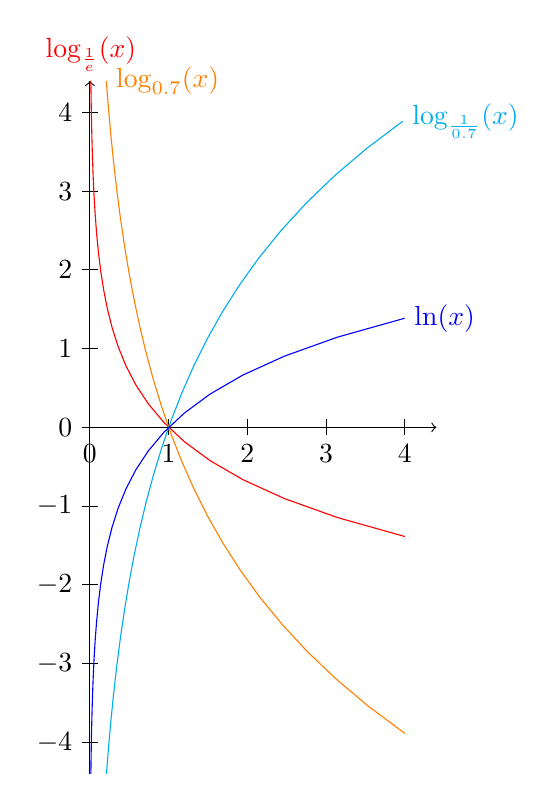
\begin{tikzpicture}[]
\draw[arrows=->] (0,0) -- (4.4,0) node[below] {$\R$};
\draw[arrows=->] (0,-4.4) -- (0,4.4) node[left] {$\R$};
\foreach \pos in {0,1,2,3,4}
    \draw[shift={(\pos,0)}] (0,.1) -- (0,-.1) node[below] {$\pos$};
\foreach \pos in {-4,-3,-2,-1,0,1,2,3,4}
    \draw[shift={(0,\pos)}] (.1,0) -- (-.1,0) node[left] {$\pos$};
\draw[color=red,domain=-1.386:4.4]    plot (0.36789^\x,\x)             node[above] {$\log_{\frac{1}{e}}(x)$};
\draw[color=orange,domain=-3.887:4.4]    plot (0.7^\x,\x)             node[right] {$\log_{0.7}(x)$};
\draw[color=cyan,domain=-4.4:3.887]    plot (1.426^\x,\x)             node[right] {$\log_{\frac{1}{0.7}}(x)$};
\draw[color=blue,domain=-4.4:1.386]    plot (e^\x,\x)             node[right] {$\ln(x)$};
\end{tikzpicture}
\end{center}

Cada una de las propiedades de la exponencial se traducen en propiedades del logaritmo, solo necesitamos excluir el caso $b=1$ pues en ese caso la exponencial no es invertible y por lo tanto el logaritmo no existe.

\begin{prop}
Dado $b \in \R^+\setminus\{1\}$, se cumplen las siguientes propiedades.
\begin{enumerate}
\item[1.] $\log_b(b)=1\wedge \log_b(1)=0$
\item[2.] $\forall r,s\in\R_+,\  \log_b(rs)=\log_b(r)+\log_b(s)$
\item[3.1] $\forall r\in\R_+,\ \forall x\in\R,\  \log_b(r^x)=x\log_b(r)$
\item[3.2] $\forall r\in\R_+,\  \log_b(r)=\frac{\log_a(r)}{\log_a(b)}$
\item[4.1] $\forall r\in\R_+,\  \log_b\left(\frac{1}{r}\right)=-\log_b(r)$
\item[4.2] $\forall r\in\R_+,\  \log_{\frac{1}{b}}(r)=-\log_b(r)$
\item[5.] $\forall r,s\in\R_+,\  \log_b\left(\frac{r}{s}\right)=\log_b(r)-\log_b(s)$
\end{enumerate}
\end{prop}
{\bf Demostración.} Sea $b \in \R^+\setminus\{1\}$ cualquiera.
\begin{enumerate}
\item[1.] $\log_b(b)=1\Leftrightarrow b=\exp_b(1)\Leftrightarrow b=b^1\Leftrightarrow b=b$.
\item[2.] Sean $r,s\in\R_+$, y sean $u=\log_b(r)$ y $v=\log_b(s)\in\R$.
Esto equivale a decir que $b^u=r$ y $b^v=s$.
Usamos la propiedad 2 de la exponencial y obtenemos que 
\begin{align*} 
b^{u+v}=b^ub^v&\Leftrightarrow b^{u+v}=rs\\
&\Leftrightarrow \log_b(rs)=u+v\\
&\Leftrightarrow \log_b(rs)=\log_b(r)+\log_b(s)
\end{align*}

\item[3.1] Sea $x\in\R$, $r\in\R_+$, y sea $u=\log_b(r)\in\R$.
Esto equivale a decir que $b^u=r$.
Usamos la propiedad 3 de la exponencial y obtenemos que 
\begin{align*} 
(b^{u})^x=b^{xu}&\Leftrightarrow b^{xu}=r^x\\
&\Leftrightarrow \log_b(r^x)=xu\\
&\Leftrightarrow \log_b(r^x)=x\log_b(r)
\end{align*}

\item[3.2] 
Sea $a \in \R^+\setminus\{1\}$, $r\in\R_+$, y sean $u=\log_a(b)$, $v=\log_b(r)\in\R$.
Esto equivale a decir que $a^u=b$ y $b^v=r$.
Usamos la propiedad 3 de la exponencial y obtenemos que 
\begin{align*} 
(a^{u})^v=a^{vu}&\Leftrightarrow a^{vu}=b^v=r\\
&\Leftrightarrow \log_a(r)=vu\\
&\Leftrightarrow \log_a(r)=\log_b(r)\log_a(b)\\
&\Leftrightarrow \log_b(r)=\frac{\log_a(r)}{\log_a(b)}
\end{align*}

\item[4.1] Sea $r\in\R_+$ de las propiedades anteriores, se cumple:
\begin{align*}
\log_b\left(\frac{1}{r}\right)&=\log_b(r^{-1})\\
&=-\log_b(r)\\
\end{align*}

\item[4.2] Sea $r\in\R_+$ y sea $u=\log_b(r)\in\R$, de las propiedades anteriores, se cumple:
\begin{align*}
\log_{\frac{1}{b}}(r)=u&\Leftrightarrow \left(\frac{1}{b}\right)^u=r\\
&\Leftrightarrow r^{-1}=b^u\\
&\Leftrightarrow u=\log_b(r^{-1})\\
&\Leftrightarrow u=-\log_b(r)\\
&\log_{\frac{1}{b}}(r)=-\log_b(r)\\
\end{align*}

\item[5.] Sean $r,s\in\R_+$ de las propiedades anteriores, se cumple:
\begin{align*}
\log_b\left(\frac{r}{s}\right)&=\log_b(rs^{-1})\\
&=\log_b(r)+\log_b(s^{-1})\\
&=\log_b(r)-\log_b(s)\\
\end{align*}
\hfill $\Box$
\end{enumerate}

Especialmente útil es la llamada fórmula del cambio de base (ítem 3.2):

$$\log_b(r)=\frac{\log_a(r)}{\log_a(b)}$$

Nos permite calcular un logaritmo en una base usando sus valores en otra base, por ejemplo:

$$\log_5(8)=\frac{\ln(8)}{\ln(5)}\sim 1,292.$$

Pero también nos permite expresar una exponencial en una base en términos de otra base, simplemente agragando una constante multiplicativa al exponente:

$$ a^x=(e^{\ln(a)})^x=e^{\ln(a) x}.$$

Dado que $\ln(a)$ es constante, no varía con $x$, la función $e^{\ln(a) x}$ es la composición de una exponencial con una recta, la exponencial $e^x$ con la recta $\ln(a)x$.
Esto demuestra que toda exponencial es la composición de una exponencial en la base que más me guste con una recta.

Veamos ahora algunas importantes aplicaciones de la exponencial y el logaritmo.

\begin{enumerate}
\item Suponga que un Banco me ofrece hacer un dep\'osito
			plazo fijo de $K_0$ pesos por 2 a\~nos con una tasa de inter\'es
		del $11.4$ porciento ($q = 0.114$) .
		Despu\'es de 2 a\~nos tendr\'e entonces $K(1) = K_0(1+q)$.
		Si decido dejar mi dinero en el dep\'osito a plazo por 2 a\~nos m\'as,
		tendr\'e luego de esos 2 a\~nos $K(2) = K(1)(1+q) = K_0(1+q)^2$.
		Si esto se repite $m$ veces, despu\'es de $2m$ a\~nos, mi capital
		ser\'a de $K(m) = K_0(1+q)^m$.
		Ahora quiero calcular cu\'antas veces debo renovar mi dep\'osito a 
		plazo si quiero esperar hasta que mi capital inicial de $K_0$ pesos se 
		haya duplicado.
		Quiero entonces encontrar $m_0$ (debo renovar mi
		dep\'osito a plazo $m_0-1$ veces ) de modo que $K(m_0) = K_0(1+q)^{m_0} = 2K_0$.
		\[
				K_0(1+q)^{m_0} = 2K_0 \gdw (1+q)^{m_0} = 2 \gdw
				\log_{1+q}(2) = m_0 \gdw m_0 = \frac{\log(2)}{\log(1+q)}.
		\]
		Ahora bien, con esta ecuación probablemente obtendré $m\not\in\N$, pero entonces tomo el entero más pequeño que sea mayor al número obtenido, esto me asegurará al menos doblar mi capital:
		$$m_0 = \left\lceil\frac{\log(2)}{\log(1.114)}\right\rceil=\left\lceil6.42\right\rceil=7$$
		Debo renovar el depósito 6 veces, es decir, invertir por 14 años seguidos.
\item El {\em tiempo medio de vida} de una sustancia radioactiva es 
		igual a $C$, esto significa que, si $M_0$ es la cantidad
		inicial de la sustancia, despu\'es de $C$ unidades de
		tiempo, quedar\'an $\frac{M_0}{2}$ unidades de ella.
		As\'{\i}, despu\'es de $nC$ unidades de tiempo, la cantidad
		que queda de la sustancia ser\'a $M(n) = M_0\left(\frac 1 2\right)^n$.
		Quiero calcular despu\'es de cu\'antas unidades de tiempo
		la cantidad que quede de la sustancia que considero es 
		un d\'ecimo de la cantidad original, es decir, 
		quiero encontrar $n_0$ de modo que 
		\[
			\frac{M_0}{10} = M_0\left(\frac 1 2\right)^{n_0}
				\gdw \frac{1}{10} = \left(\frac 1 2\right)^{n_0}
				\gdw n_0 = \log_{\frac 1 2}\frac{1}{10}.
		\]
		Es decir, $n_0 = \log_{\frac 1 2}10^{-1} = -\log_{\frac 1 2}(10) = 
		\log_2(10)=\frac{\log(10)}{\log(2)}=\frac{1}{\log(2)}\sim3.322$.
		Lo cual nos dice que pasadas aproximadamente $3.322C$ unidades de tiempo la sustancia habrá disminuido a la décima parte.
\item El nivel de ruido $d$ de un sonido se calcula en {\em decibeles (dB)} y depende de la potencia $W$
		del sonido seg\'un la f\'ormula
		\[
			d(W) = 10\log\dfrac{W}{W_0},
		\]
		en la que $W_0$ es un valor de referencia. Un sonido con potencia igual a $W_0$ se denomina sonido umbral.
		Esto significa que un sonido umbral produce tiene $d(W_0)=10\log1=0$ decibeles.
		
		Un sonido de 20 decibeles corresponde a una potencia $W$ que cumple la ecuación:
		$$20= 10\log\dfrac{W}{W_0}$$
		Desoejando obtenemos:
		\begin{eqnarray*}
		2&=&\log\dfrac{W}{W_0}\quad \exp(\cdot)\\
		10^2&=&\dfrac{W}{W_0}\quad \times W_0\\
		100W_0&=&W
		\end{eqnarray*}
		
		Si deseamos mantener un nivel de decibeles entre -30 y 30, debemos lograr que la potencia cumpla las siguientes inecuaciones.
		$$-30\le 10\log\dfrac{W}{W_0}\le 30$$
		Dado que la función exponencia en base 10 es monótona creciente, podemos aplicarla a ambos lados de cada inecuación, sin que la desigualdad se vea afectada, entonces obtenemos las siguientes inecuaciones:
		$$10^{-3}\le \dfrac{W}{W_0}\le 10^3$$
		Por lo tanto,
		$$0.001W_0\le W\le 1000W_0.$$
\item El sism\'ologo F. Richter (1900-1985) ide\'o en
		1935 la {\em escala de Richter} que compara la fuerza de los terremotos.
		Seg\'un esta escala la magnitud $R$ de un terremoto se define como
		\[
			R = \log\left(\frac{A}{A_0}\right),
		\]
		donde $A$ es la amplitud de la onda s\'{\i}smica mayor, y $A_0$ es una
		amplitud de referencia. % y $C$ es una constante.
		La magnitud del terremoto de Concepci\'on, del 
		27 de febrero de 2010, fue de $8.8$ en la escala de Richter, mientras
		que el terremoto de Iquique del 1 de abril de 2014 fue de magnitud $8.2$.
		\footnote{La escala de Richter ya no se usa, así que los valores dados no son exactos, por otra parte la fórmula que aquí se presenta es solo una simplificación de la verdadera fórmula de la magnitud de Richer, la cual contempla otros factores, tales como la duración del sismo, sin embargo el ejercicio sirve como una primera aproximación apara sopesar qué significan los grados de la escala de Richter y otras escalas sísmicas.}.

		Esto nos dice que:
		$$A=A_010^R$$

		Si llamamos $A_I$ a la amplitud de la onda del sismo de Iquique y $A_C$ a la del sismo de Concepción, podemos calcular que:
		$$\frac{A_C}{A_I}=\frac{A_010^{8.8}}{A_010^{8.2}}=\exp(0.6)=10^{0.6}\sim 3.981$$
		En otras palabras, el terremoto de Concepción fue aproximadamente 4 veces más fuerte que el de Iquique.
\item La catenaria es la curva que forma un cable al colgar libremente, sostenido por dos soportes a igual altura.
Corresponde al también conocido como \emph{coseno hiperbólico}, $\textup{cosh}: \R \to \R$, cuya fórmula está dada por 
		\[
			\textup{cosh}(x) = \frac{e^x + e^{-x}}{2}.
		\]
		
		Podemos observar que esta función es par, no es inyectiva ni sobreyectiva, y en 0 vale 1.

\end{enumerate}


